% -----------------------------------------------
% Template for ISMIR Papers
% 2015 version, based on previous ISMIR templates
% -----------------------------------------------

\documentclass{article}
\usepackage{ismir,amsmath,cite}
\usepackage{graphicx}
\usepackage{color}

% Title.
% ------
\title{Four Difficult Lessons on Automatic Chord Estimation}

% Two addresses
% --------------
%\twoauthors
%  {First author} {School \\ Department}
%  {Second author} {Company \\ Address}

% Three addresses
% --------------
\threeauthors
  {First author} {Affiliation1 \\ {\tt author1@ismir.net}}
  {Second author} {\bf Retain these fake authors in\\\bf submission to preserve the formatting}
  {Third author} {Affiliation3 \\ {\tt author3@ismir.net}}


\begin{document}
%
\maketitle
%
\begin{abstract}

Automatic chord estimation (ACE) is now a hallmark research topic in content-based music informatics, but like many other tasks, system performance appears to be converging to yet another glass ceiling.
Recently, two different large-vocabulary ACE systems were developed in the hopes that complex, data-driven models might significantly advance the state of the art.
While arguably achieving some of the highest results to date, both approaches plateau at the same level, well short of having solved the problem.
Therefore, this work explores the behavior of these two systems as a means of understanding obstacles and limitations in chord estimation, arriving at four difficult lessons:
one, music recordings that invalidate tacit assumptions about harmony and tonality result in erroneous and even misleading performance;
two, standard lexicons and comparison methods struggle to reflect the natural relationships between chords;
three, conventional approaches conflate the competing goals of recognition and transcription to some undefined degree;
and four, the perception of chords in real music can be highly subjective, making the very notion of ``ground truth'' annotations tenuous.
Synthesizing these observations, this paper offers possible remedies going forward, and concludes with some perspectives on the future of ACE research.

\end{abstract}




\section{Introduction}\label{sec:introduction}

% Chord rec is standard in the community
Among the various subtopics in content-based music informatics, automatic chord estimation (ACE) has matured into a prototypical MIR challenge, receiving healthy attention from the research community for the better part of two decades.
 % benchmark challenge at the annual MIReX event\footnote{{http://www.music-ir.org/mirex/wiki/MIREX\_HOME}}.
%, people want / need
Complementing our healthy sense of academic intrigue, the broader music learning public places a high demand on chord-based representations of popular music, as evidenced by large online communities surrounding websites like e-chords\footnote{http://www.e-chords.com} or Ultimate Guitar\footnote{http://www.ultimate-guitar.com}.
% Countless individuals invest considerable time and effort in the curation and consumption of popular music transcriptions,
% ...but this is difficult
However, given the prerequisite skill necessary to manually identify chords from recorded audio, there is considerable motivation to develop automated systems capable of reliably performing this task.

Following these motivations, the goal of an ACE system is --or, at least, has been-- to produce ``good'' time-aligned sequence of chords from a given music signal.
% We've stepped up to the challenge, and have been revising our designs.
Notably, most approaches to the task adopt the same basic architecture, diagrammed in Figure \ref{fig:basic_ace} \cite{Cho2014Improved}:
first, harmonic features, referred to as pitch class profiles (PCP) or \emph{chroma}, are extracted from short-time observations of the audio signal \cite{Fujishima1999Realtime};
these features may then be processed by any number of means, referred to in the literature as \emph{pre-filtering};
next, \emph{pattern matching} is performed independently over observations to measure the similarity between the signal and a set of pre-defined chord classes, yielding a time-varying posterior likelihood;
and finally, \emph{post-filtering} is applied to this chord class posterior, resulting in a sequence of chord labels over time.


% We've been hacking at this for a while though, and we're noting some diminsing returns
% Some refine features
% Some have thrown bigger beastlier models at it
% Some have tried feature learning
% Some have mixed all the things
Recently, in an effort to continue to advance the state of the art, researchers have begun exploring more complex post-filtering methods such as Dynamic Bayesian Networks (DBNs) \cite{Mauch2010Approximate}, Conditional Random Fields \cite{Sumi2012Music}, Variable-Length Markov Models \cite{Chordia2011Predictive}, or Recursive Neural Networks \cite{Boulanger2013Automatic}.


% Not just about building a better mousetrap
% Been curating data
% Developing syntax
% Discussing evaluation
%


\section{But what is a ``chord''?}

% Attempts to define a chord
a \emph{chord} is classically conceived as a simultaneous grouping of notes.
While much of this theory can be detailed specifically, real music is by no means so well behaved.
As a result, a more practical definition of a ``chord'' is open to some interpretation, and may take multiple meanings.
For example, \cite{McVicar2013Machine} collects three possible definitions, restated here:

\begin{enumerate}
\item \emph{Everyone agrees that \emph{chord} is used for a group of musical tones.}
\item \emph{Two or more notes sounding simultaneously are known as a chord.}
\item \emph{Three or more pitches sounded simultaneously or functioning as if sounded simultaneously.}
\end{enumerate}

% Pitch and notes
Additionally, \cite{Harte2010Towards} expands the scope of (2) in order to describe \emph{all} tonal music, ``allow[ing] a chord to comprise zero or more notes.''
The various flavors of definitions begs an obvious question: what makes the concept of a chord so hard to pin down?

% Chord composition
Much of this difficulty stems from the fact that the relative importance of the individual notes in a collection may change in different contexts.
In practice, a chord is named based on three, potentially subjective, criteria:
its root, its contributing intervals, and how these two relate to the perceived key.
Therefore, as will be shown shortly, a chord may take a different name if any of these decisions are changed or re-weighted.

% Why is it so hard to define a chord? Let's look at some examples

% Expanded over time leads to the same chord
A coarse understanding of the variation inherent to defining a chord can be obtained by exploring a few simple examples.
The one invariant property shared by all definitions named previously is the idea that a pitch collection may be understood as a single harmonic object.
The time span over which this phenomena may unfold, however, is flexible.
To illustrate the point, consider the three bars notated in Figure \ref{fig:expanded_major}, where a major chord is written as a true simultaneity, an arpeggiation, and as an series of non-overlapping quarter notes, respectively.
In this instance, the degree of overlap in time is expanded until it no longer exists, and yet the collection of notes continues to function as a coherent harmonic object.

\begin{figure}[t]
\centering
\includegraphics[width=0.8\textwidth]{expanded_major}
\caption{A stable F major chord played out over three time scales, as a true simultaneity, an arpeggiation, and four non-overlapping quarter notes.}
\label{fig:expanded_major}
\end{figure}

\begin{figure}[t]
\centering
\includegraphics[width=0.6\textwidth]{nonchord_tones}
\caption{A stable C major chord is embellished by passing non-chord tones.}
\label{fig:nonchord_tones}
\end{figure}

% True simultaneity doesn't always make a chord
On the other hand, as shown in Figure \ref{fig:nonchord_tones}, the simultaneous sounding of different notes does not necessarily give rise to the perception of different chords.
Here, a major triad is sustained under the first several degrees of its scale.
While three notes in the upper voice are contained in the C-major triad, the others --the D, F, and A-- are referred to as ``nonchord'' tones.
These extra notes are explained away in the overall harmonic scene, as they fall on metrically weak beats, are comparatively short in duration, and quickly move to notes that \emph{are} in the chord.
These embellishments do not contribute to the harmonic center of the phrase, and the bar can still be understood as a stable C major chord.




\section{Methodology}


\subsection{Data}\label{subsec:data}

In order to objectively measure the quality of a proposed ACE system, it is necessary to address two related components: the collection of ground-truth data, and the manner in which estimations are compared to this reference data.

The first major effort to curate ground truth chord transcriptions was led by Harte in the mid-2000s, referred to as the Isophonics dataset\footnote{\url{http://isophonics.net/content/reference-annotations}}, where a small team of researchers transcribed the entire discography of The Beatles.
Containing chord annotations for 180 tracks, this was a landmark dataset in the field of MIR and shaped years of ACE research.
Importantly, this transcription effort leveraged professional transcriptions of the music under consideration, and was verified for accuracy multiple times.
However, despite this rigor, the data is drawn from a single artist and very well known to the research community; some have argued that ACE research has begun to manually overfit this collection.

To combat these issues, two datasets were released following the 2011 Conference of the International Society of Music Information Retrieval (ISMIR), one of over 700 tracks led by J. Ashley Burgoyne \cite{Burgoyne2011Expert} and another of 295 tracks led by Tae Min Cho, from the Music and Audio Research Lab at NYU\footnote{\url{https://github.com/tmc323/Chord-Annotations}}; here, the former is referred to as ``Billboard'' and the latter as ``MARL-Chords'', corresponding to their related projects.
In parallel, an additional, comparatively small, dataset was released, containing 20 tracks by the band Queen, provided by Matthias Mauch as an extension to the Isophonics set.
In all four cases, the chord transcriptions are provided as ``ground truth'', on the premise that the data corresponds to the expert perspective.
To help prevent errors and resolve judgment calls, these additional annotation efforts employed a review process, where the transcriptions of one or more annotators were verified by a different individual.

Thirteen chord qualities, given in Table \ref{tab:qualities}, in all twelve pitch classes and one no-chord class are considered for a total of 157 chord classes.
Having all four datasets at hand, these collections are merged into the largest collection of chord transcriptions used to date, totaling 1235 tracks.
Given that the collections were curated in isolation of each other, it is a necessary first step to identify and remove duplicates to avoid data contamination during cross validation.
To these ends, each recording is checked against the EchoNest Analyze API\footnote{http://developer.echonest.com/docs/v4} and associated with its track and song identifiers, corresponding to the recording and work, respectively.
Though multiple track IDs will map to the same song ID, uniqueness is defined at the level of a song to ensure duplicates are removed.
This identifies 18 redundant songs, and all but one is dropped for each collision from the total collection, resulting in a final count of 1217 unique tracks.


\subsection{Automatic Systems}

For algorithmic parity, two systems are considered here having adopted the same output chord prediction space and trained over the same data splits.


\subsubsection{K-stream GMM-HMM with Multiband Chroma}

Following the lineage of automatic chord estimation systems, one system considered is that of \cite{Cho2014Improved}.
A multiband chroma representation is computed from beat-synchronous audio analysis, producing four parallel chroma features.
Each is fit to a separate Gaussian Mixture Model (GMM) by rotating all chroma vectors and chord labels to C.
During inference, four separate observation likelihoods over all chord classes are obtained by circularly rotating the feature vector the GMM.
These four posteriors are then decoded jointly, using a k-stream HMM, resulting in a beat-aligned chord sequence.
In addition to being one of the highest performing systems at a recent iteration of MIReX, a software implementation was obtained, thereby enabling experimental consistency between partitions of the training data.


\subsubsection{Deep Convolutional Neural Network}

Acknowledging both the limited representational power of GMMs and a similar trend that occurred in automatic speech recognition, a deep convolutional network is also considered \cite{Humphrey2015Fully}.
Time-frequency patches of local contrast normalized constant-Q spectra, on the order of one second, are transformed by a fully-convolutional network.
Finding inspiration in the root-invariance strategy of GMM training, explicit weight-tying is achieved across roots such that all qualities develop the same internal representations, allowing the model to generalize to chords unseen during.

DNN


\subsection{Evaluation}

Expressed formally, the conventional approach to scoring an ACE system is a weighted measure of chord-symbol recall, $R_{W}$, between a reference, $\mathcal{R}$, and estimation, $\mathcal{E}$, chord sequence as a \emph{continuous} integral over time, summed over a collection of $N$ pairs:

\begin{equation}
\label{eq:recall_micro}
R_{W} = \frac{1}{S}\sum_{n=0}^{N-1}\int_{t=0}^{T_n}C(\mathcal{R}_n(t), \mathcal{E}_n(t))~dt
\end{equation}

\noindent Here, $C$ is a chord \emph{comparison} function, bounded on $[0, 1]$, $t$ is time, $n$ the index of the track in a collection, $T_n$ the duration of the $n^{th}$ track. $S$ corresponds to the cumulative amount of time, or \emph{support}, on which $C$ is defined, computed by a similar integral:

\begin{equation}
S = \sum_{n=0}^{N-1}\int_{t=0}^{T_n}(\mathcal{R}_n(t), \mathcal{E}_n(t) \in \Re)~dt
\end{equation}

Defining the normalization term $S$ separately is useful when comparing chord names, as it relaxes the assumption that the comparison function is defined for all possible chords.
Furthermore, setting the comparison function as a free variable allows for flexible evaluation of a system's outputs, and thus all emphasis can be placed on the choice of comparison function, $C$.
In practice, this measure has been referred to as \emph{Weighted Chord Symbol Recall} (WCSR) \cite{Harte2010Towards}, \emph{Relative Correct Overlap} (TCO) \cite{McVicar2013Machine}, or \emph{Framewise Recognition Rate} \cite{Cho2014Improved}, but it is, most generally, a recall measure.

As discussed, most ACE research typically proceeds by mapping all chords into a smaller chord vocabulary, and using an enharmonic equivalence comparison function at evaluation, e.g. \texttt{C\#:maj} == \texttt{Db:maj}.
Recently, this approach was generalized by the effort behind the open source evaluation toolbox, \texttt{mir\_eval} \cite{Raffel2014Eval}, introducing a suite of chord comparison functions.
The seven rules considered here are summarized in Table \ref{tab:mir_eval}.

\begin{table}[t]
\begin{center}
\caption{Chord comparison functions and examples in \texttt{mir\_eval}.}
\label{tab:mir_eval}
\begin{tabular}{l | c | c | c }
Name & Equal & Inequal & Ignored \\
\hline
Root & \texttt{G\#:aug}, \texttt{Ab:min} & \texttt{C:maj/5}, \texttt{G:maj} & -- \\
Thirds & \texttt{A:maj}, \texttt{A:aug} & \texttt{C:maj7}, \texttt{C:min} & --\\
Triads & \texttt{D:dim}, \texttt{D:hdim7} & \texttt{D:maj}, \texttt{D:aug} & -- \\
Sevenths & \texttt{B:9}, \texttt{B:7} & \texttt{B:maj7}, \texttt{B:7} & \texttt{sus2}, \texttt{dim} \\
Tetrads & \texttt{F:min7}, \texttt{F:min(b7)} & \texttt{F:dim7}, \texttt{F:hdim7} & -- \\
majmin & \texttt{E:maj}, \texttt{E:maj7} & \texttt{E:maj}, \texttt{E:sus2} & \texttt{sus2}, \texttt{dim} \\
MIREX & \texttt{C:maj6}, \texttt{A:min7} & \texttt{C:maj}, \texttt{A:min} \\
\hline
\end{tabular}
\end{center}
\end{table}

The meaning of most rules may be clear from the table, but it is useful to describe each individually.
The ``root'' comparison only considers the enharmonic root of a chord spelling.
Comparison at ``thirds'' is based on the minor third scale degree, and is equivalent to the conventional mapping of all chords to their closest major-minor equivalent.
In other words, a chord with a minor-third is minor, e.g. $\texttt{dim7} \to \texttt{min}$, and \emph{all} other chords map to major, e.g. $\texttt{sus2} \to \texttt{maj}$.
The ``triads'' rule considers the first seven semitones of a chord spelling, encompassing the space of major, minor, augmented, and diminished chords.
The ``sevenths'' rule is limited to major-minor chords and their tetrad extensions, i.e. major, minor, and dominants;
chords outside this set are considered ``out-of-gamut'' and ignored.
The ``tetrads'' comparison extends this to all chords contained within an octave, e.g. six chords and half-diminished sevenths.
The ``Major-minor'' comparison is limited to major and minor chords alone;
like ``sevenths'', other chords are ignored from evaluation.
Unlike the other rules, ``MIREX'' compares chords at the pitch class level, and defines equivalence if three or four notes intersect.
Comparing the pitch class composition of a chord allows for a slightly relaxed evaluation, allowing for misidentified roots and related chords.
Finally, rules that ignore certain chords only do so when they occur in a reference annotation.
In other words, an estimation is not held accountable for chords deemed to be out of gamut, but predicting such chords is still counted as an error.



\section{Observations, in Four Parts}\label{sec:typeset_text}

Based on this analysis, a handful of instances are pulled out of the data and inspected more closely.

% Content Validity
\subsection{Harmonic Validity}\label{subsec:body}

Not all music is well described by chords.
Because you \emph{can} annotate chords in a song, doesn't mean you should.
Revolution 9, Beastie Boys, Fugees.
These are not well described by chords, and introduce noise in the evaluation process.

Alternatively, systems are sensitive to tuning.
This is another easy way to pick up goose eggs during evaluation.
While the outputs might be spot on and even useful to a human, sensitivity to absolute chord spelling fails to
This motivates harmonic, Roman numeral analysis as a slightly different formulation of the task; decouple tuning from function.
While not all chord datasets contain this information, Billboard and Isophonics do.

Within the realm of all Western music, the use of harmony and chords has steadily evolved over time.
Classically, music theorists have long sought to characterize musical works via analysis and reduction as a means to understanding, typically operating from a symbolic representations, i.e. a score.
As a result, the language of ``chords'' developed as an expressive, yet compact, language with which one might describe a piece of music harmonically.
However, Western ``pop music'', infused with elements of folk, blues, jazz, rock and countless other influences, is not to required to adhere to or consider the rules of traditional tonal theory \cite{Tagg1982Analysing}.
Thus efforts to understand the former in the language of the latter is ultimately limited by the validity in doing so.

While contemporary popular music is certainly influenced by this tradition, it by no means adheres to the same rules and conventions.
Even in the constrained space of Western tonal music set forth here, not all musical works will be well-described by the language of harmonic analysis, and thus chords may be a clumsy language with which to describe such music.
An alternative approach to analysis, such as voice leading, might make more sense in this instance;
in others, such as ``math rock'', a lack of clearly structured harmonic content may arguably render the goal of harmonic analysis irrelevant \cite{Cateforis2002Alternative}.
As genre is itself an amorphous and ill-defined concept, the degree to which a piece of music might be understood harmonically will vary, both absolutely and internally.



\subsection{The Significance of Chord Representations}

% Syntax yo
As discussed in \ref{sec:chord_syntax}, it is a particular nuance of chord notation that the space of valid spellings is effectively infinite.
To constrain the complexity of the task at hand, ACE systems are traditionally designed to estimate chords from a finite \emph{vocabulary}, defined \emph{a priori}.
This simplification reduces the chord estimation to a classification problem, where all observations are assigned to one of $K$ chord \emph{classes}.

Comparing chords in label space is bonkers.
Mappings or resolutions effectively quantize chords to a one-hot encoding.
These can be thought of as mapping chords to bit vectors and then testing for equivalence.
This is the wrong representation.

One, chords are inherently hierarchical, and this approach to resolution discards these relationships.
Flat classification problems ---those in which different classes are conceptually independent--- are built on the assumption of mutually exclusive relationships.
In other words, assignment to one class precludes the valid assignment to any other classes considered.
For example, ``cat'' and ``dog'' are mutually exclusive classes of ``animal'', but ``cat'' and ``mammal'' are not.
Returning to chords, \texttt{C:dim7} and \texttt{C:maj} are clearly mutually exclusive classes, but it is difficult to say the same of \texttt{C:maj7} and \texttt{C:maj}, as the former \emph{contains} the latter.

Two, the flexibility of the standard Harte syntax can be abused for ambiguous chords, and it isn't clear what to do with these labels.

Occurrence of bizarre chord spellings in the data:
Should these even exist?


\begin{table}[!t]
% increase table row spacing, adjust to taste
% \renewcommand{\arraystretch}{1.4}
% if using array.sty, it might be a good idea to tweak the value of
% \extrarowheight as needed to properly center the text within the cells
\small
\caption{Various real chord transcriptions for ``With or Without You'' by U2, comparing the reference annotation with six interpretations from a popular guitar tablature website; a raised asterisk indicates the transcription is given relative to a capo, and transposed to the actual key here.}
\label{tab:wowu_chords}
\centering
\begin{tabular}{ c || c c c c | c c c c |}
Ver. & \multicolumn{4}{c}{Chord Sequence} & Score & Ratings & Views \\
 \hline
Ref. & \texttt{D:maj} & \texttt{D:maj/5} & \texttt{D:maj6/6} & \texttt{D:maj(4)/4} & --- & --- & --- \\
\hline
1 & \texttt{D:maj} & \texttt{A:maj} & \texttt{B:min} & \texttt{G:maj} & 4/5 & 193 & 1,985,878 \\
2 & \texttt{D:5} & \texttt{A:sus4} & \texttt{B:min7} & \texttt{G:maj} & 5/5 & 11 & 184,611 \\
$3^*$ & \texttt{D:maj} & \texttt{A:maj} & \texttt{B:min} & \texttt{G:maj} & 4/5 & 23 & 188,152 \\
$4^*$ & \texttt{D:maj} & \texttt{A:maj} & \texttt{B:min} & \texttt{G:maj7} & 4/5 & 14 & 84,825 \\
$5^*$ & \texttt{D:maj} & \texttt{A:maj} & \texttt{B:min} & \texttt{G:maj} & 5/5 & 248 & 338,222 \\
6 & \texttt{D:5} & \texttt{A:5} & \texttt{D:5/B} & \texttt{G:5} & 5/5 & 5 & 16,208 \\
\hline
\end{tabular}
\end{table}

Chords with bass intervals other than the root should be discarded from chord mapping strategies.
Otherwise, this will only introduce noise.


\subsection{The Internal Conflict between ``Recognition'' and ``Transcription''}

The former is literal, the latter is anything but.
In a recognition problem, silence is always no-chord, because nothing is playing.
Transcription, on the other hand, is attempting to assign labels to regions, and is closer to segmentation than classic approaches to chord estimation.
It is easy to find instances of both in the data.

Unfortunately, reference datasets contain annotations of both styles, and sometimes internally to the same annotation.
Over-specified chords are mostly indicative of a recognition problem, and finds an ambiguous middle ground between harmonic analysis and pitch recognition.
Alternatively, there are plenty of instances in which annotators make transcriptions decisions.
Nirvana -- all apologies.


\subsection{``There is No Spoon,'' or the  }

Known issue, Ni and company.
Not enough attention is being drawn to this observation.
How can we objectively quantify a subjective task?

Examples in the data




\section{First Level Headings}

First level headings are in Times 10pt bold,
centered with 1 line of space above the section head, and 1/2 space below it.
For a section header immediately followed by a subsection header, the space should be merged.

\subsection{Second Level Headings}

Second level headings are in Times 10pt bold, flush left,
with 1 line of space above the section head, and 1/2 space below it.
The first letter of each significant word is capitalized.

\subsubsection{Third and Further Level Headings}

Third level headings are in Times 10pt italic, flush left,
with 1/2 line of space above the section head, and 1/2 space below it.
The first letter of each significant word is capitalized.

Using more than three levels of headings is highly discouraged.


\section{Footnotes and Figures}

\subsection{Footnotes}

Indicate footnotes with a number in the text.\footnote{This is a footnote.}
Use 8pt type for footnotes. Place the footnotes at the bottom of the page on which they appear.
Precede the footnote with a 0.5pt horizontal rule.

\subsection{Figures, Tables and Captions}

All artwork must be centered, neat, clean, and legible.
All lines should be very dark for purposes of reproduction and art work should not be hand-drawn.
The proceedings are not in color, and therefore all figures must make sense in black-and-white form.
Figure and table numbers and captions always appear below the figure.
Leave 1 line space between the figure or table and the caption.
Each figure or table is numbered consecutively. Captions should be Times 10pt.
Place tables/figures in text as close to the reference as possible.
References to tables and figures should be capitalized, for example:
see \figref{fig:example} and \tabref{tab:example}.
Figures and tables may extend across both columns to a maximum width of 17.2cm.

\begin{table}
 \begin{center}
 \begin{tabular}{|l|l|}
  \hline
  String value & Numeric value \\
  \hline
  Hello ISMIR  & \conferenceyear \\
  \hline
 \end{tabular}
\end{center}
 \caption{Table captions should be placed below the table.}
 \label{tab:example}
\end{table}

\begin{figure}
 \centerline{\framebox{
 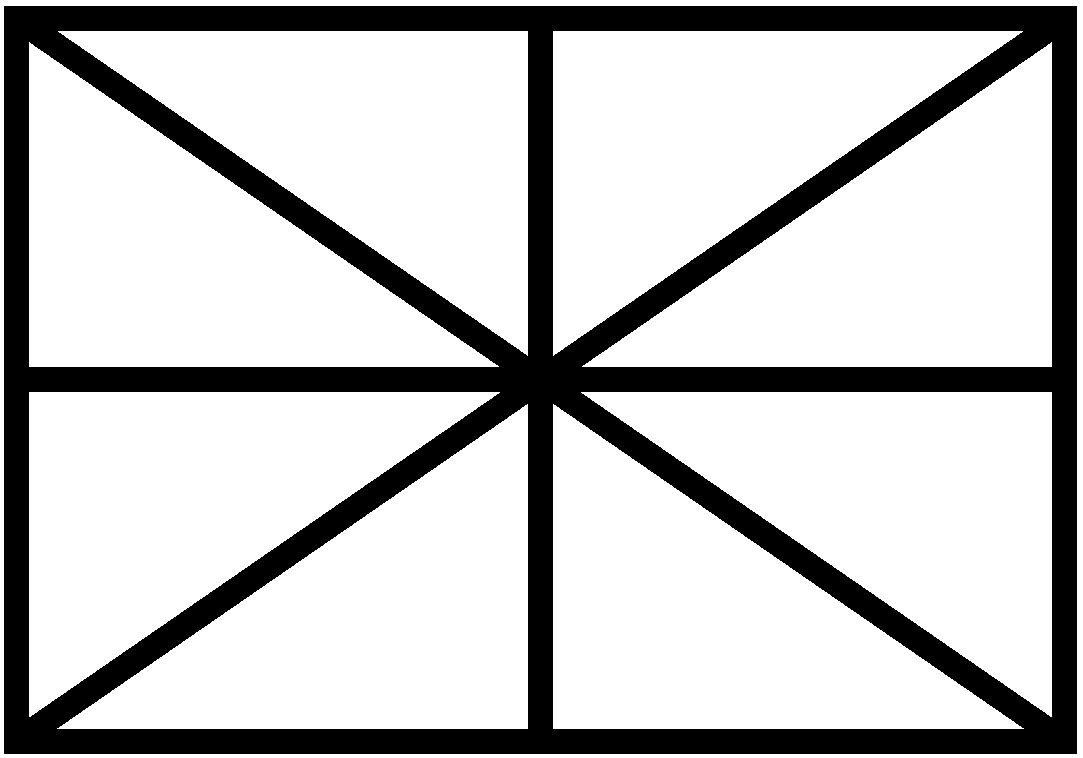
\includegraphics[width=\columnwidth]{figure.png}}}
 \caption{Figure captions should be placed below the figure.}
 \label{fig:example}
\end{figure}

\section{Conclusions}

In this work, the application of deep learning to large-vocabulary ACE is thoroughly explored, advancing the state of the art using standard evaluation methods.
Arguably of more importance, both the behavior of the resulting systems and the data used for development are explored in rigorous detail.
Our results show that the state of the art may have truly hit a glass ceiling, due to the conventional assumption that ``ground truth'' data can be obtained for what is, at times, an unavoidably subjective task.
This challenge is further compounded by approaches to prediction and evaluation, which attempt to perform flat classification of a hierarchically structured chord taxonomy.
Thus, while there certainly remains room for improvement, error analysis indicates that the vast majority of error in modern chord recognition systems is a result of invalid assumptions baked into the very question being asked.

Notably, four issues with current chord estimation methodology have been identified in this work.
One, it seems necessary that computational models, and especially those that estimate a large number of chord types, embrace structured outputs;
one-of-$K$ class encoding schemes introuduce unnecessary complexity between what are naturally hierarchical relationships.
Two, there is value in distinguish between the two tasks at hand, being chord recognition ---I am playing this \emph{exact} chord shape on guitar--- and chord transcription ---finding the best chord label to describe this harmonically homogenous region of music--- and how this intent is conveyed to the authors of reference annotations.
Three, as championed by \cite{Mauch}, chord transcription would certainly seem to benefit from explicit segmentation, rather than letting such boundaries between regions of harmonic stability result implicitly from post-filtering algorithms, i.e. Viterbi.
Lastly, the all-too-often subjective nature of chord labeling needs to be acknowledged in the process of curating reference data, and the human labeling task should average or combine multiple perspectives rather than attempt to yield canonical ``expert'' references.


% \section{Citations}

% All bibliographical references should be listed at the end,
% inside a section named ``REFERENCES,'' numbered and in alphabetical order.
% All references listed should be cited in the text.
% When referring to a document, type the number in square brackets
% \cite{Author:00}, or for a range \cite{Author:00,Someone:10,Someone:04}.

% For bibtex users:
\bibliography{ISMIR2015template}

% For non bibtex users:
%\begin{thebibliography}{citations}
%
%\bibitem {Author:00}
%E. Author.
%``The Title of the Conference Paper,''
%{\it Proceedings of the International Symposium
%on Music Information Retrieval}, pp.~000--111, 2000.
%
%\bibitem{Someone:10}
%A. Someone, B. Someone, and C. Someone.
%``The Title of the Journal Paper,''
%{\it Journal of New Music Research},
%Vol.~A, No.~B, pp.~111--222, 2010.
%
%\bibitem{Someone:04} X. Someone and Y. Someone. {\it Title of the Book},
%    Editorial Acme, Porto, 2012.
%
%\end{thebibliography}

\end{document}
